\section*{Источники и решения}

\subsubsection*{Покер: быстрый вопрос}

Этим вопросом меня озадачил Стэн Уэгон, а он нашёл его в книге Аарона Фридланда \cite{18}.

Суть в том, что все \emph{фулл-хаусы} с тремя тузами одинаково сильны, ведь из одной колоды двух таких не набрать.
Однако фулл-хаусы бьются другими комбинациями: любое \emph{каре}, а их 11 штук, и, что важнее для нас, \emph{стрит-флэшами}.
Фулл-хаусы ТТТ99, ТТТ88, ТТТ77 и ТТТ66 выбивают из колоды максимальное число стрит-флэшей.
Каждый туз выбивает два стрит-флэша, а каждая фоска (карта младшего достоинства) выбивает по пять --- всего 16.
Эти фулл-хаусы и являются лучшими.

Если же взять ТТТКК, то вас побьют $40 - 9 \z= 31$ стрит-флэшей, или даже $40 - 16 = 24$, если в вашем фулл-хаусе не оказалось всех четырёх мастей.

\subsubsection*{Восстановление многочлена}

Эту загадку мне подкинул Джо Булер (Рид-колледж), который считает, что она должна быть очень древней.

Как вы, наверно, догадались, достаточно двух запросов:
если $p(1)\z=n$, то коэффициенты не превышают $n$.
Далее можно взять $x = n + 1$, записать ответ $(n + 1)$-ичной системе счисления, и получить все коэффициенты многочлена!

Джо отметил, что если бы разрешалось использовать произвольные числа, то хватило бы одного запроса $x = \pi$.
Надо думать, что Оракул найдёт способ выдать значение $p(\pi)$ за конечное время;
если же вместо этого он станет выдавать его десятичное разложение по одной цифре, то вам придётся понять, когда остановиться.

Хельге Тверберг обратил внимание на то, что эта задача имеет смысл для многочленов с неотрицательными вещественными коэффициентами.
Чтобы восстановить $p$, сначала спросим $p(1)$; если ответ $0$, то $p = 0$ и задача решена.
В противном случае будем строить \emph{конечные разности}.
Положим $p_0(x) = p(x)$, и определим рекурсивно последовательность многочленов $p_{i+1}(x) = p_i (x+1) - p_i(x)$.
Отметим, что коэффициенты всех $p_i$-х неотрицательны.
За $k$ вопросов получим $p(1),\dots,p(k)$,
а из них вычислим $p_{k-1}(1)$.
Наименьшее $k$ при котором мы получим $0$ это $d+2$, где $d$ --- степень $p$.
Как только мы знаем $d$, любых $d+1$ из имеющихся у нас $d+2$ значений достаточно, чтобы восстановить многочлен.

\subsubsection*{Спасите наши души}

На эту игру мне указала аспирантка Рэйчел Эссельштейн.
Наряду с другими играми, она обсуждается в книге Тома Фергюсона по теории игр \cite{ferguson}.
Этот вариант игры также предлагался на 28-й Американской математической олимпиаде 1999 года.

Вопрос выглядит туманным, пока не поймёшь, что единственный способ вынудить противника сделать проигрывающий ход, --- это заставить его ходить внутрь конфигурации S-пусто-пусто-S (мы будем называть её \emph{ямой}).
Например, Тристан может выиграть, если $n = 7$, поставив $S$ в середину, а затем поставив ещё одну $S$ в конце, подальше от ответного хода Изольды.
Теперь у нас есть яма.
После пары ходов на другой стороне Изольде придётся сходить в яму и проиграть.

То же самое справедливо для любого нечётного $n$ больше $7$ --- Тристану достаточно поставить $S$ в такую клетку, чтоб осталось не меньше 4 клеток с обеих сторон, построить яму с одной из сторон, и ждать.

Если $n$ чётное, то у Тристана нет шансов, ведь Изольде не могут достаться одни ямы --- каждый раз она выбирает из нечётного числа пустых клеток.
Если же $n$ чётное и большое, то Изольда выигрывает, поставив $S$ далеко от концов и от первого хода Тристана.
Однако, если Тристан начинает с $O$, то Изольде нельзя поставить $S$ рядом, поэтому потребуется дополнительное место.

Для случая $n = 14$, если Тристан поставит $O$ на $7$-ю клетку (нумерация от $1$ до $14$), то лучший ответ Изольды --- $S$ на $11$-ю клетку (угроза ямы с $S$ на $14$-й клетке).
В ответ Тристан может поставить $O$ на $13$-ю или $14$-ю клетку (или $S$ на $12$-ю). 
Теперь Изольда хотела бы построить яму, ставя $S$ на $8$-ю клетку, но ей нельзя, ведь тогда Тристан выиграет, поставив $S$ на $6$-ю.

Таким образом, при $n = 14$ --- ничья;
Изольде нужно, чтобы $n$ было чётным и не менее 16.
В итоге, Тристан выигрывает, если $n$ --- нечётное и не менее $7$,
Изольда --- если $n$ --- чётное и не меньше $16$.
При всех остальных значениях $n$ получаем ничью при оптимальной игре.

\subsubsection*{Пасьянс с шарами}

Эту головоломку (немного в другом виде) можно найти в книге Мартина Гарднера \cite[2.16]{30}, однако там ответ дан без доказательства.
Доказательство из упомянутой там статьи \cite{45} занимает три страницы и оно слишком сложное как для Гарднеровской книги, так и для моей.

К счастью, есть простой способ понять, что вероятность выигрыша всегда равна $1/2$, независимо от соотношения красных и зелёных шаров в урне.
Ниже приведено рассуждение Серджио Харта из Иерусалимского университета, который и обратил моё внимание на эту задачу.

Часто при анализе случайного процесса полезно перетащить случайность в другое место.
В этой задаче допустимо думать, что перед каждым раундом оставшиеся шары случайно упорядочиваются, и после этого выбираются слева направо.
Тогда в последнем раунде все шары одноцветны.
В предыдущем раунде есть шары обоих цветов, но все красные шары стоят слева, а все зелёные справа, или наоборот.
Независимо от числа шаров каждого цвета на этом этапе (или изначально), эти два порядка равновероятны.
Поскольку первый приводит к выигрышу, а второй к проигрышу, получаем, что вероятность выигрыша равна 1/2.

Серджиу обратил внимание на то, что этот пасьянс в некотором смысле эквивалентен «Потерянному посадочному талону» \cite[стр. 42]{59}.
Хельге Тверберг (Бергенский университет в Норвегии) отметил, что есть также не столь хитрое, но вполне изящное решение индукцией по числу шаров.

\subsubsection*{Пиратская демократия}

Об этой старой загадке мне напомнил аспирант Дартмутского университета Джулио Дженовезе.
Как и многие игры, она решается обратным ходом.
Пронумеруем пиратов от младшего к старшему, и пока будем считать, что у них всего $n$ монет.
Если дело дойдёт до самого младшего $P_1$, то он, конечно же, возьмёт всё золото себе. Будем надеяться, что он сможет довести корабль к пристани!

Однако, если дело дошло до $P_1$, то оно дошло и до $P_2$, а
$P_2$, конечно же, оставит себе все монеты и проголосует «за», останется в живых и возглавит корабль.

Далее, если дело дошло до $P_3$, то он купит голос $P_1$ за одну монету, взяв оставшиеся $n - 1$ себе.
Следовательно, наилучшим вариантом для $P_4$ будет подкупить $P_2$ одной монетой --- этого достаточно, ведь иначе тот не получит ничего.

$P_5$ нужны уже два голоса, и он получит их, отдав по монете $P_1$ и $P_3$, --- этого достаточно.

Уже есть что доказывать индукцией:
если осталось нечётное число пиратов, то следует предложить по одной монете каждому оставшемуся нечётному пирату (предполагая, что монет хватит);
если же их чётное число, то следует предложить по одной монете каждому оставшемуся чётному пирату.
По предположению индукции, все получающие монеты пираты проголосуют «за», и уже нечего доказывать.

Так что там по поводу капитана?
Чтобы точно выжить, ему потребуется 49 монет; дабы предложить по монете всем чётным пиратам ниже 100.

\begin{addedbytheeditors}
Итак, 49 монет хватает.
Может показаться, что лучшего добиться нельзя.
Однако на самом деле меньшего количества тоже хватает.

Давайте продолжим рассуждение.
Предположим в кладе всего 48 монет.
Этого хватает для выживания $P_{98}$, но уже не хватает $P_{99}$: против любого его плана проголосуют те 50 пиратов, которым ничего не достаётся.
Следовательно, $P_{99}$ будет голосовать за любое предложение капитана, лишь бы не отправится за борт.
Значит, капитан получит два бесплатных голоса, свой и от $P_{99}$ и сможет купить ещё 48 голосов --- этого хватает.   

Рассуждая таким образом, можно показать, что капитан выживает если команды размера $2n+2^k$, где $n$ --- запас монет, а $2^k$ --- любая степень двойки.
Таким образом, минимальный достаточный для выживания капитана запас монет будет решением уравнения $2n+2^6=100$, то есть $n=18$.
(Заметим, что при $19$ монетах, капитану не выжить.) 

В квантовской заметке  Сергея Грибка и Константина Кнопа \cite{gribok-knop} разобрано около десятка вариаций этого сюжета;
в пятой задаче денег для дележа меньше, чем нужно для подкупа всех чётных пиратов.
\pr
\end{addedbytheeditors}


\subsubsection*{Волшебные рамки}

Эту головоломку предложил Эхуд Фридгут из Еврейского университета; похожая задача была на израильском молодёжном математическом соревновании.
В соревновании рамки были размером $3 \times 3$ и $4 \times 4$.
В этом случае подсчёт вариантов говорит, что всех конфигураций цветов достичь невозможно.
Суть в том, что порядок, в котором располагаются рамки, не имеет значения;
достаточно знать, какими способами установки рамок мы воспользовались.
У нас есть $5^2$ способов установки рамки $4 \times 4$
и $6^2$ способов установки рамки $3 \times 3$.
Таким образом, всего $2^{25} \times 2^{36} = 2^{61}$ варианта — этого мало.

Однако в варианте Фридгута у нас уже $2^{49} \times 2^{36}$ вариантов, и теоретически этого хватает для получения всех $2^{64}$ конфигураций.
Думаете, теперь получится?

\begin{figure}[ht!]
\centering
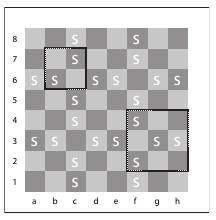
\includegraphics[scale=1]{pics/chess}
\caption{Особые клетки (помечены буквой S) и пара рамок.}
\label{pic:chess1}
\end{figure}

Назовём клетку \emph{особой}, если она находится в третьей или шестой строке, или в третьем, или шестом столбце, но не в обоих таких позициях сразу (рис. \ref{pic:chess1}).
Тогда каждая рамка $2 \times 2$ или $3 \times 3$ покрывает чётное число особых клеток.

Поскольку изначально на доске чётное число чёрных особых клеток, мы не сможем достичь конфигурации с нечётным  числом чёрных особых клеток.

\subsubsection*{Больше рамок на меньшей доске}

Эту головоломку подкинул мне Джулио Дженовезе.
Он узнал её от Владимира Чернова, тренировавшего Джулио к Олимпиаде Патнема; сам Владимир нашёл её в книге «Новые олимпиады по математике» \cite{markova}.

Как и в предыдущей задаче, нужно найти чудесный инвариант.
Однако давайте проверим другой подход, и убедимся, что он не работает.

Конечно же, достаточно рассматривать только рамки $2 \times 2$, $3 \times 3$ и $5 \times 5$, ведь из них составляются все остальные.

Как уже было отмечено, стоит проверить, хватит ли всего того, что \emph{разрешается}, для того чтобы сделать всё, что \emph{нужно}.
Можно думать, что номера на доске --- это числа по модулю $3$ ($0$, $1$ или $2$, и $2 + 1 = 0$).
Следовательно, нам надо беспокоиться о $3^{6^2} = 3^{36}$ возможных конфигурациях.
На каждой клетке доски каждый тип квадрата может быть установлен, не установлен или установлен дважды; установка трижды ничего не даёт.
У нас $5^2$ мест для установки квадрата $2 \times 2$,
$4^2$ для $3 \times 3$
и $2^2$ для $5 \times 5$, так что в общей сложности есть $3^{25} \times 3^{16} \times 3^4 = 3^{45}$ возможных действий, и этого более чем достаточно.
Очевидно, многие из этих действий дают один и тот же результат.
Так или иначе, пока неясно, доступны ли все конфигурации.

Математически говоря, у нас есть линейное отображение из векторного пространства $\mathbb{Z}_3^{45}$ в векторное пространство $\mathbb{Z}_3^{36}$, и мы хотим узнать покрывает ли его образ всё $\mathbb{Z}_3^{36}$.
(Возможность перехода от конфигурации со всеми нулями к любой произвольной конфигурации эквивалентна обратному.)

Если ответ да, то можно перейти от всех нулей к конфигурации, со всеми нулями, кроме одной единицы в выбранной клетке.
Более того, если такое возможно, то задача решена, ведь можно проделать это для каждой клетки, которой не хватает единицы, и дважды для клетки, которой не хватает двойки.
Это напоминает поиск решения (с нуля) для кубика Рубика --- нужны операции, которые мало чего меняют.
Например, начнём с двух диагонально сдвинутых квадратов $3 \times 3$, перекрывающихся по квадрату $2 \times 2$.
Теперь, если добавить по два подквадрата $2 \times 2$ в каждый угол квадрата $4 \times 4$ и ещё два центральных квадрата, то всё отменится, кроме двух диагонально противоположных углов квадрата $4 \times 4$.
Таким образом, можно увеличить на единицу числа в паре клеток, одна из которых находится в трёх шагах от другой по диагонали.

Однако сложно представить, что можно изменить одно значение в произвольной клетке.
Давайте сменим цель.
Допустим это \emph{не так}, то есть невозможно получить любую конфигурацию.
Тогда должен найтись \emph{инвариант}: некоторое число, связанное с конфигурацией, которое ни для какого шага не меняется.
В линейной задаче подобного рода этот инвариант сам должен быть линейной функцией.
Это означает, что должно быть два таких подмножества клеток $A$ и $B$, что если сложить числа в $A$ и прибавить удвоенную сумму чисел в $B$ (в нашей арифметике по модулю $3$ это то же, что сумма чисел в $A$ минус сумма чисел в $B$), то получим инвариант.

\begin{figure}[t!]
\centering
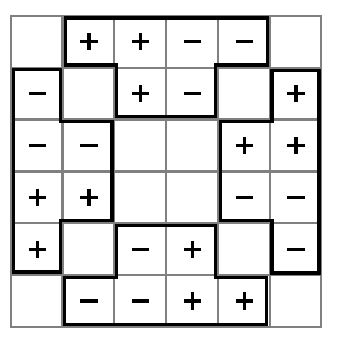
\includegraphics[scale=1]{pics/chess2}
\caption{Множества $A$ и $B$ помечены знаками $+$ и $-$.}
\label{pic:chess2}
\end{figure}

Из построения выше, для любой клетки из $A$, клетка в трёх шагах от неё по диагонали (всегда есть ровно одна такая) находится в $B$, и наоборот.
Исходя из этого наблюдения и зная, что нам нужно в каждой возможной рамке равное число клеток в $A$ и в $B$ (по модулю 3), придумывается чудесный узор, показанный на рис. \ref{pic:chess2}, в котором точки в $A$ помечены плюсами, а точки в $B$ --- минусами.
Итак, мы утверждаем, что сумма значений в клетках с плюсами, минус сумма значений в клетках с минусами, не меняется.
Отсюда следует, что мы не можем перейти от любой позиции, где это значение не равно $0$, к позиции, в которой все значения равны~$0$.

\begin{addedbytheeditors}
Эта задача предлагалась ученикам 8 классов на одной из олимпиад Украины в 1990-х годах, откуда и попала в книгу \cite{markova}, однако нам пока не удалось отыскать более точную информацию.
\pr
\end{addedbytheeditors}

\subsubsection*{Простой блеф}

Эта головоломка была предложена Джереми Торпом и Луизой Фуше из Калифорнийского технологического института, но похожие игры были известны и раньше.

Отметим, что, имея на руках пику, Луиза всегда выгодно поднимать ставку.
Поэтому у неё есть две \emph{чистые} стратегии:
\begin{itemize}
 \item \textbf{честная} --- поднимать ставку только если есть пика.
 \item \textbf{нахальная} --- всегда поднимать ставку.
\end{itemize}
Если Луиза подняла ставку, то у Джереми есть два варианта ответа:
\begin{itemize}
 \item \textbf{робкий} --- сбросить.
 \item \textbf{смелый} --- проверить.
\end{itemize}

Вероятность вытянуть пику составляет $1/4$.
Значит, честная стратегия против робкой даёт Луизе 1 доллар в $1/4$ ставок, а остальных 1 доллар выигрывает Джереми.
Ожидаемый выигрыш Джереми составит $1/2$ доллара.
Честная стратегия против смелой даёт Луизе 11 долларов, если у неё пика,
а в среднем приносит ей 2 доллара ($\tfrac14 \times 11 - \tfrac 34 \times 1 = 2$).

Далее, нахальная стратегия против робкой приносит Луизе 1 доллар каждый раз,
в то время как нахальная против смелой обходится ей в $5{,}50$ долларов в среднем ($\tfrac34 \times 11- \tfrac14 \times11 = 5{,}50$).
Если вставить эти числа в матрицу игры $2 \times 2$,
то мы не увидим доминирующей стратегии ни для одного из игроков.
Значит, как и следовало ожидать, придётся использовать смешанную (вероятностную) стратегию.

Из работ Джона фон Неймана (ещё до Джона Нэша) известно, что существует \emph{равновесие Нэша} для этой игры --- пара стратегий, при которых ни один из игроков не может улучшить свою стратегию, при условии, что другой игрок не меняет свою.
Посмотрим, что это означает для Луизы: если ей не выгодно переходить к честной или нахальной стратегии, то в среднем ей всё равно, проверит ли её Джереми или сбросит.

Предположим, что Луиза решила блефовать с вероятностью $p$, если у неё нет пики.
Против робкой стратегии её ожидаемый выигрыш в среднем составит $\tfrac14 \times 1 + p \times \tfrac34 \times 1 - (1 - p) \times \tfrac34 \times 1 =(\tfrac32p - \tfrac12)$,
ну а против смелой, $\tfrac14 \times 11 - p \times \tfrac34 \times 11 - (1 - p) \times \tfrac34 \times 1 \z= (2 - \tfrac{15}2p)$ долларов.

Поскольку Луизе должно быть всё равно, эти две величины обязаны совпасть, и значит $p = 5/18$.
То есть, Луизе следует блефовать $5$ раз из $18$, когда у неё нет пики и, конечно, всегда повышать ставку, если пика есть.
Её ожидаемый выигрыш независимо от стратегии Джереми будет
\[\frac32\times\frac5{18}-\frac12=2-\frac{15}2\times\frac5{18}=-\frac1{12}\]
долларов.
То есть в среднем Луиза теряет по $\tfrac1{12}$ доллара за игру.

Немного поразмыслив, убеждаемся, что Луизе выгодно увеличение ставки,
однако в среднем она останется в минусе, если, конечно, игра ведётся честно.
Причина в том, что если у неё нет пики, то она не может позволить себе блефовать чаще, чем один раз из трёх.
Иначе, с точки зрения Джереми, вероятность того, что у неё была бы пика, составила бы не больше половины, и поэтому Джереми мог бы просто всегда проверять.
Луиза в лучшем случае выйдет в ноль при повышениях ставки, и будет терять по доллару без повышений, а значит, в среднем будет проигрывать.
Но если $p < 1/3$, то Луиза проигрывает робкой стратегии Джереми;
в этом случае она чаще теряет свою ставку, чем выигрывает.

Здесь важно, что вероятность вытянуть пику составляет одну четверть.
Если бы шансы были чуть выше (скажем, если бы в колоде не хватало дамы червей), то б\'{о}льшая ставка повернула бы удачу на сторону Луизы.

Вернёмся к исходным 10 долларам.
Давайте вычислим стратегию равновесия для Джереми (хотя нам этого и не требуется).
Положим, что Джереми проверяет с вероятностью $q$ когда Луиза повышает ставку.
Тогда, против луизиной честной стратегии, он получает $\tfrac34 \times 1 \z- \tfrac14 \times q \times 11 \z- \tfrac14 \times (1 - q) \times 1 \z= \tfrac12 \z- \tfrac52q$ долларов,
а против смелой стратегии $\tfrac34 \times q \times 11 \z- \tfrac14 \times q \times 11 \z- (1 - q) \times 1 \z= \tfrac{13}2q \z- 1$ долларов.
Полагая, что эти величины равны, получаем $q = \tfrac3{18}$.
То есть, Джереми должен проверять только $\tfrac3{18}$ всего времени.
Подстановка $q = \tfrac3{18}$ обратно в выражения даёт Джереми $\tfrac1{12}$ доллара выигрыша за игру в среднем, как и должно быть, ведь ровно столько теряет Луиза.

\subsubsection*{Китайский Ним}

Эта игра известна как китайский ним, или ним  Витхоффа;
она появилась в его статье 1907 года \cite{60}.
Игра обсуждается несколько раз в первом и втором томе классической книги Элвина Берлекэмпа, Джона Конвея и Ричарда  Гая \cite{4}.
Связь с уже рассмотренной задачей про надёжные мигалки была замечена в прекрасной книге Сергея Табачникова \cite{56}.
Однако ни одна из этих книг не приводит вывод стратегии.

Каждая позиция $\{x, y\}$ в игре либо выигрышная, либо проигрышная для игрока, который начинает, при условии оптимальной игры обоих.
Как и в классическом ниме, проще всего попытаться описать проигрышные позиции, поскольку их меньше.

Как только известны проигрышные позиции, можно вывести правильную стратегию.
Если, например, Алекс находится в выигрышной позиции, то у него должна быть возможность одним ходом перейти к проигрышной позиции для Бет.
Если же Алекс находится в проигрышной позиции, то он может только надеяться на ошибку Бет, или же он по-джентльменски предложит ей сделать первый ход.
Таким образом, стратегия сводится к списку проигрышных позиций.
Но разве здесь нет порочного круга?
Разве нам не нужно знать правильную стратегию, чтобы найти проигрышные позиции?
К счастью, поскольку число бобов всегда уменьшается, можно начать снизу и постепенно подниматься вверх.

\begin{figure}[!b]
\vskip-0mm
\centering
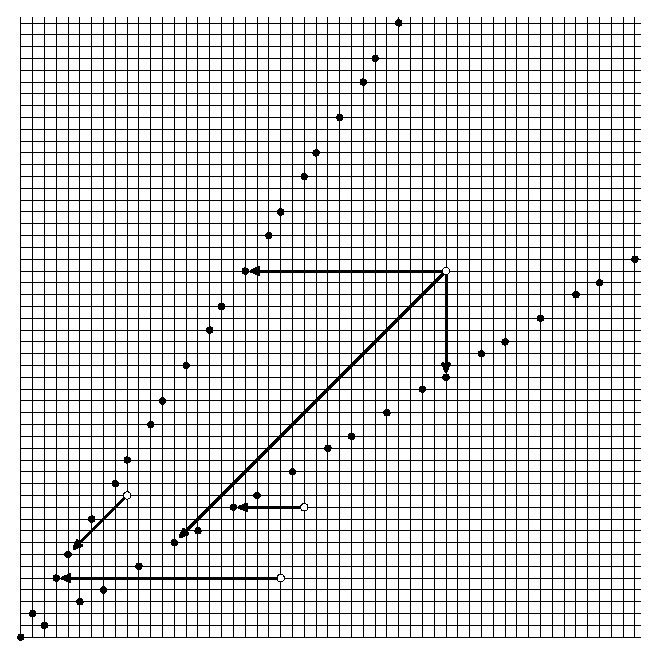
\includegraphics{mppics/pic-5}
\vskip-0mm
\caption{Проигрышные позиции и несколько выигрышных ходов.}
\label{pic:nim}
\end{figure}

Любая позиция с одной пустой кучей или с кучами одинакового размера автоматически выигрышная.
Не сложно понять, что самая простая проигрышная позиция --- это $\{1, 2\}$.
После этого можно увидеть, что $\{3, 5\}$, $\{4, 7\}$ и $\{6, 10\}$ также проигрышные.
Но где же закономерность?

Пусть $\{x_1 , y_1\}$, $\{x_2 , y_2\},\dots$ будут проигрышными позициями для первого игрока (не считая $\{0, 0\}$);
мы предполагаем, что $x_i < y_i$ и $x_i < x_j$ при $i < j$.
Заметим, что $x_i \ne x_j$ для $i \ne j$, ведь если $x_i = x_j$, то Алекс мог бы сделать ход от большего из $y_i$ и $y_j$ к меньшему, оставляя Бет в проигрышной позиции --- противоречие.

Немного поразмыслив, приходим к выводу, что если известны все проигрышные позиции от $\{x_1 , y_1\}$ до $\{x_{n-1}, y_{n-1}\}$, то $x_n$ есть наименьшее положительное число, которого нет среди чисел из $\{x_1, \dots , x_{n-1}\} \z\cup \{y_1, \dots , y_{n-1}\}$, а $y_n = x_n + n$.
В этом случае $y_n$ больше любого числа из $\{x_1, \dots , x_{n-1}\} \cup \{y_1, \dots , y_{n-1}\}$.

Доказательство ведётся индукцией по $n$.
Мы уже знаем, что $x_n$ не может быть среди чисел в $\{x_1, \dots , x_{n-1}\} \cup \{y_1, \dots , y_{n-1}\}$, а также, что не может быть более одного $y_n$, который соответствует этому $x_n$.
Остаётся показать, что позиция $\{x_n, y_n\}$ проигрышная.

Если $\{x_n, y_n\}$ была бы выигрышной, то из неё можно было бы прийти в $\{x_i, y_i\}$ для некоторого $i < n$; но такой позиции нельзя достичь, уменьшив меньшую кучу или уменьшив обе кучи на одинаковое число бобов, ведь это сделало бы разницу между двумя кучами $n$ или больше.
Также нельзя её достичь, уменьшив б\'{о}льшую кучу, ведь тогда был бы ещё один игрек для одного икса.
Таким образом, $\{x_n, y_n\}$ проигрышная.

Теперь можно получить список проигрышных позиций любой длины.
Из этого легко вывести стратегию Алекса.
Если он столкнётся с $\{x_i , y_i\}$, он возьмёт один-два боба, надеясь на ошибку.
Если он видит $\{x_i , z\}$ для $z > y_i$, он уменьшает $z$ до $y_i$.
Если он видит $\{x_i , z\}$ с $x_i < z < y_i$, то есть разница $d = z - x_i < i$, он берет из обеих куч, чтобы дойти до $\{x_d , y_d\}$ (если $z = y_j$ для некоторого $j < i$, то у него также есть вариант уменьшить $x_i$ до $x_j$).
Если он видит $\{y_i , z\}$ с $y_i \le z$, то может уменьшить $z$ до $x_i$, а может иметь и другие варианты.


Однако, подсчёт всех проигрышных позиций, скажем, до тысячи бобов в каждой куче требует значительных усилий.
Можно ли найти более явное их описание?

Как мы уже знаем, $x_n$ лежит между $n$ и $2n$ для каждого $n$, ведь $x_n$ стоит сразу после всех $x_i$ и некоторых $y_i$ при $i < n$.
Разумно предположить, что $x_n$ примерно равно $rn$, для некоторого $r$ между $1$ и $2$.
Если это так, то $y_n$ примерно равно $rn + n = (r + 1)n$.

Если это подтвердится, то $n$ иксов между $1$ и $x_n$ примерно равномерно распределены, и, следовательно, доля $r/(r + 1)$ от их числа будет соответствующих игрекам ниже $x_n$.
Таким образом, у нас около $nr/(r + 1)$ игреков ниже $x_n$, и вместе с $n$ иксами, всего получается $x_n$ чисел; то есть
\[n+n\frac{r}{r+1}=nr,\]
что даёт нам $r + 1 = r^2$ или $r = (1 + \sqrt{5})/2$ --- знакомое \emph{золотое сечение}.

Наверное, теперь к вам на ум пришло блестящее наблюдение --- поскольку $r$ иррационально и $\tfrac1r+\tfrac1{r^2}=1$, числа $r$ и $r^2$($= r + 1$) подходят на роль $p$ и $q$ в решении «Надёжных мигалок» из главы 3.
Как мы знаем, любое положительное целое число представимо единственным способом \emph{либо} как $\lfloor pm\rfloor$ для некоторого целого $m$, \emph{либо} как $\lfloor qn\rfloor$ для некоторого целого $n$.

А теперь уже возникает подозрение, что $x_n=\lfloor rn\rfloor$, а $y_n=\lfloor r^2 n\rfloor$.
Конечно же, эти значения обладают желаемыми свойствами:
каждое $x_n$ --- наименьшее положительное число, не из $x_1, \dots , x_{n-1}$ или $y_1, \dots, y_{n-1}$, иначе его было бы невозможно получить.
Остаётся проверить, что $\lfloor r^2 n\rfloor - \lfloor rn\rfloor = n$, но это легко, ведь $r^2 n - rn$ равно целому числу $n$,
поэтому и разница их целых частей обязана быть $n$ --- готово!

Забавы ради, давайте найдём ход Алекса из предложенных примеров.
Обратите внимание, что $12 000/r$ чуть меньше $7417$, и $7417r \z= 12 000{,}9581\dots$ так что $12 000$ это один из иксов, точнее $x_{7417}$.
Соответствующее значение $y_{7417}$ равно $\lfloor 7417r^2\rfloor = 19 417$, поэтому если в другой куче $20 000$ бобов, Алекс может выиграть, забрав из неё $20 000 \z- 19 417 = 583$ боба.
Если же в другой куче всего $19 000$ бобов, то Алекс может выиграть, уменьшив кучи одновременно до $\{x_{7000}, y_{7000}\} \z= \{11 326, 18 326\}$.

\begin{addedbytheeditors}
Эта игра известна также под названием «цзяньшицзы».
Ей посвящена, в частности, квантовская статья Альгирдаса Матулиса и Альгимантаса Савукинаса \cite{matulis-savukinas}.
Удобное описание проигрышных позиций получается также в \emph{фибоначчиевой системе счисления}, см. \cite[задача 129]{yaglom-yaglom} или
\cite[разделы 6.6---6.7]{graham-knut-patashnik}.\pr
\end{addedbytheeditors}
